\apendice{Especificación de Requisitos}

\section{Introducción}

Los requisitos \cite{req:info} que ha de satisfacer una aplicación pueden ser vistos como las cláusulas de un contrato entre el cliente y la empresa desarrolladora del programa. La especificación de requisitos software describirá cómo debe comportase el sistema que desea el cliente. Esta especificación ha de incluir un conjunto de casos de uso (requisitos funcionales) describiendo las interacciones que el usuario puede tener con el sistema. También se han de incluir los requisitos no funcionales ya que implican restricciones en la implementación del software.

Es importante que la citada especificación de requisitos sea de fácil comprensión para el cliente y el equipo de desarrollo.

Así mismo se recomienda seguir un conjunto de buenas prácticas sugeridas por el estándar IEEE 830-1998 \cite{ieee:info}. Estas son:

\begin{itemize}
	\item \textbf{Completa:} se incluirán todos los requerimientos.
	\item \textbf{Consistente:} la ERS debe ser coherente con los requerimientos y con la documentación usada durante la implementación.
	\item \textbf{Inequívoca:} no debe dejarse lugar a la mal interpretación de la misma.
	\item \textbf{Correcta:} el producto desarrollado ha de ceñirse a los requisitos detallados.
	\item \textbf{Trazable:} debiendo poder identificar todos los requisitos.
	\item \textbf{Priorizable:} los requisitos podrán ser organizados según su prioridad.
	\item \textbf{Modificable:} la modificación de los requisitos debe ser sencilla. 
	\item \textbf{Verificable:} existiendo una forma de comprobar que todo lo aquí mencionado se cumple de forma verídica.
\end{itemize}

Como ha sido comentado anteriormente, es posible identificar dos tipos de requisitos:

\begin{itemize}
	\item \textbf{Requisitos funcionales:} son los que se encuentran relacionados con los casos de uso, determinan qué servicios proporciona el sistema al usuario.
	\item \textbf{Requisitos no funcionales:} determinan las restricciones de diseño o implementación del sistema.
\end{itemize}


En este anexo se incluyen los apartados necesarios para describir los requisitos de esta aplicación.

\section{Objetivos generales}

Los objetivos generales que se han llevado a cabo durante el desarrollo de este Trabajo de Fin de Máster son los siguientes:

\begin{enumerate}
	\item Desarrollo de una aplicación que permita gestionar todos los aspectos necesarios para el análisis de rutas basadas en coordenadas geográficas.
	\item Desarrollo de un algoritmo que permita incorporar la información de paradas y Puntos De Interés a las rutas que se van a incorporar al sistema.
	\item Asignación de semántica (PDIs) a las paradas detectadas por el algoritmo de análisis de rutas.
	\item Diseño de una interfaz de usuario sencilla y de fácil manejo, adaptable a distintos formatos de pantalla.
\end{enumerate}

\section{Catalogo de requisitos}
A partir de los objetivos generales marcados en el apartado anterior se puede extraer tanto el conjunto de requisitos funcionales como el conjunto ligado a los requisitos no funcionales.

\subsection{Requisitos funcionales}
A continuación se detalla el listado de requisitos funcionales:

\begin{itemize}
	\item \textbf{RF-1 Gestión de datos:} La aplicación ha de poder facilitar al usuario la gestión de ficheros de datos.
	\begin{itemize}
		\item \textbf{RF-1.1 Subida de ficheros:} la plataforma contará con una sección de subida de ficheros al servidor.
		\item \textbf{RF-1.2 Borrado de ficheros:} se ha de facilitar el borrado parcial o total de los ficheros mantenidos en el servidor.
	\end{itemize}
	
	\item \textbf{RF-2 Algoritmo de análisis de rutas:} la plataforma web ha de contar con un algoritmo que permita procesar las rutas de los usuarios.
	 \begin{itemize}
		\item \textbf{RF-2.1 Búsqueda de rutas:} el algoritmo ha de permitir buscar rutas y/o seccionar una ruta en diferentes rutas dependiendo de las opciones marcadas por el usuario.
		\item \textbf{RF-2.2 Búsqueda de paradas:} una vez analizadas las rutas, el algoritmo permitirá la búsqueda de paradas dentro de cada ruta.
		\item \textbf{RF-2.3 Búsqueda de PDIs:} si la ruta analizada cuenta con paradas, el algoritmo será capaz de asignar PDIs cercanos a las rutas siguiendo las opciones del usuario.
		\item \textbf{RF-2.4 Almacenado en Base de Datos:} se ha de poder almacenar la información en una Base de Datos.
	\end{itemize}
	
	\item \textbf{RF-3 Gestión de datos:} Se ha de proporcionar una sección de gestión de los datos almacenados.
	\begin{itemize}
		\item \textbf{RF-3.1 Gestión de áreas:} la sección de gestión de datos permitirá la creación de áreas, su modificación o su eliminación.
		\item \textbf{RF-3.2 Gestión de PDIs:} la correspondiente sección de gestión de PDIs ha de proporcionar al usuario la facilidad de creación de PDIs en la Base de Datos mediante el tratamiento de ficheros xml. También permitirá el borrado o modificación de dichos PDIs.
		\item \textbf{RF-3.3 Borrado total o parcial:} la sección de borrado de datos permitirá eliminar de forma parcial o total los datos y ficheros almacenados en el servidor.
	\end{itemize}
	
	\item \textbf{RF-4 Recuperación de información:} La recuperación de la información ha de ser sencilla para el usuario inexperto.
	\begin{itemize}
		\item \textbf{RF-4.1 Tabla de pruebas:} la plataforma web contará con una tabla de pruebas ejecutadas mostrando de forma clara los parámetros de cada ejecución del algoritmo de análisis de rutas.
		\item \textbf{RF-4.2 Selección de áreas:} se facilitará la selección de áreas de tres formas diferentes.
		\begin{itemize}
			\item \textbf{RF-4.2.1 Selección unitaria:} mediante el mostrado de las áreas presentes en las tablas del sistema.
			\item \textbf{RF-4.2.2 Selección sobre mapa:} permitiendo dibujar sobre un mapa la región a seleccionar.
			\item \textbf{RF-4.2.3 Selección mediante coordenadas:} tecleando de forma manual la zona cuyas rutas se han de seleccionar.
		\end{itemize}
		\item \textbf{RF-4.3 Tabla de rutas:} se mostrará una tabla de rutas actualizada según la selección realizada sobre las áreas del sistema.
	\end{itemize}
	\item \textbf{RF-5 Mapa:} se visualizará la ruta seleccionada sobre un mapa, indicándose su inicio, PDIs hallados durante el análisis y punto final.
	\item \textbf{RF-6 Ayuda:} todas las páginas contarán con ayuda para el usuario.
\end{itemize}

\subsection{Requisitos no funcionales}
La siguiente lista permite visualizar los requisitos no funcionales:

\begin{itemize}
	\item \textbf{RNF-1 Fiabilidad:} la plataforma web ha de contar con mecanismos ante la ejecución de pruebas.
	\begin{itemize}
		\item \textbf{RNF-1.1 Ejecución de pruebas:} no se permitirá la ejecución simultánea de pruebas para mantener la coherencia de la Base de Datos.
		\item \textbf{RNF-1.2 Subida de PDIs:} no se permitirá la subida simultánea de varios ficheros de PDIs.
	\end{itemize}
	\item \textbf{RNF-2 Eficiencia:} la plataforma ha de poder ejecutarse en sistemas con un hardware limitado.
	\item \textbf{RNF-3 Facilidad de uso:} la plataforma ha de estar diseñada para todo tipo de usuarios, tanto expertos como inexpertos.
\end{itemize}

\section{Especificación de requisitos}
En la presente sección son detallados todos los casos de uso planteados.

\subsection{Diagrama de casos de uso}
El diagrama de casos de uso es el siguiente:

\begin{figure}[!htbp]
  \centering
    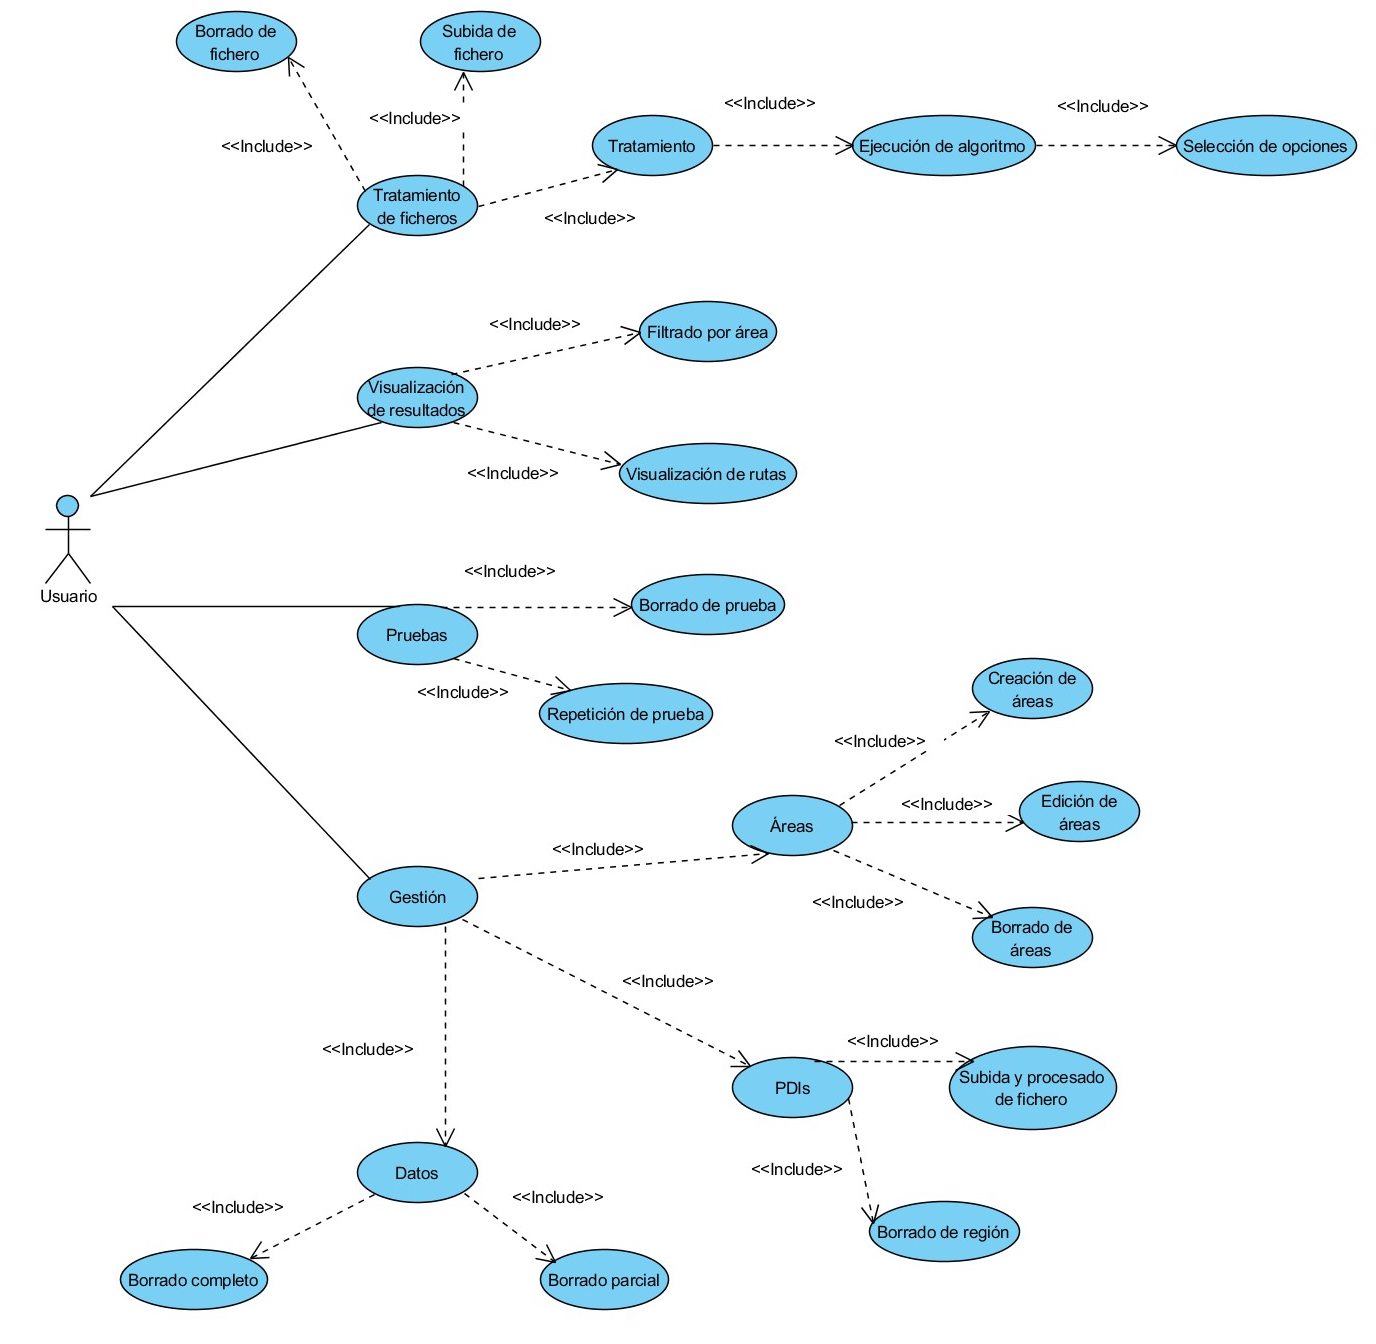
\includegraphics[width=0.8\textwidth]{../img/uml/casouso.png}
  \caption{Diagrama de casos de uso.}
  \label{casouso}
\end{figure}

\subsubsection{Actores}
Los actores son el conjunto de usuarios que pueden intervenir en el sistema desarrollado, en el caso  de esta aplicación web solo se contará con un usuario estándar:

\begin{itemize}
	\item \textbf{Usuario:} el usuario será capaz de acceder a todas las páginas de la plataforma web.
\end{itemize}


\subsubsection{Casos de uso}
A continuación se muestran las tablas descriptivas de los casos de uso del sistema.
\begin{comment}
	FICHEROS -----------------
\end{comment}

\tablaSinColores{CU-1 Subida de ficheros}
{L{3.5cm} L{10cm}}
{2}
{Tabla CU-01}
{\textbf{CU-01} & \textbf{Subida de ficheros} \\}
{\textbf{Versión} 				& 1.0\\ 
 \textbf{Autor} 				& David Moreno del Hoyo\\
 \textbf{Requisitos asociados} 	& RF-1, RF-2 \\
 \textbf{Descripción} 			& 
 La subida de ficheros implica la posibilidad de subir al servidor ficheros con rutas para ser analizados.\\
 \textbf{Precondiciones} 		& 
    \begin{itemize}
 		\item La Base de Datos está disponible.
 		\item Espacio en disco suficiente.
 	\end{itemize}
 \\
 \textbf{Acciones} 				& 
 	\begin{enumerate}
    	\item El usuario accede al sitio web.
    	\item El usuario selecciona un fichero mediante el formulario disponible.
    	\item El usuario clica sobre el botón \quotes{Enviar}.
    	\item El fichero es cargado en el sistema.
    	\item La página se refresca.
    \end{enumerate}
 \\
 
 \textbf{Postcondiciones} 		& 
    \begin{itemize}
 		\item El fichero será almacenado en el servidor.
 		\item El fichero será mostrado en la tabla de ficheros.
 	\end{itemize}
 \\
 \textbf{Excepciones} 			& 
 	\begin{itemize}
 		\item La base de datos no está disponible.
 	\end{itemize}
    
 \\
 \textbf{Importancia} 			& Alta\\}
 
  %%%%%%%%%%%%%%%%%%%%%%%%%%%%%%%%%%%%%%%%%%%%%%%%%%%%%



\tablaSinColores{CU-2 Borrado de ficheros}
{L{3.5cm} L{10cm}}
{2}
{Tabla CU-02}
{\textbf{CU-02} & \textbf{Borrado de ficheros} \\}
{\textbf{Versión} 				& 1.0\\ 
 \textbf{Autor} 				& David Moreno del Hoyo\\
 \textbf{Requisitos asociados} 	& RF-1, RF-2\\
 \textbf{Descripción} 			&  El borrado de ficheros permite borrar de forma total o parcial los ficheros del servidor.\\
 \textbf{Precondiciones} 		& 
    \begin{itemize}
 		\item La Base de Datos está disponible.
 		\item Existencia de ficheros.
 	\end{itemize}
 \\
 \textbf{Acciones} 				& 
 	\begin{enumerate}
    	\item El usuario accede al sitio web.
    	\item El usuario selecciona uno o varios ficheros existentes en el sistema.
    	\item El usuario clica sobre el botón \quotes{Eliminar}.
    	\item El fichero o ficheros son eliminados del sistema.
    	\item La página se refresca.
    \end{enumerate}
 \\
 
 \textbf{Postcondiciones} 		& 
    \begin{itemize}
 		\item El fichero se elimina.
 	\end{itemize}
 \\
 \textbf{Excepciones} 			& 
 	\begin{itemize}
 		\item La base de datos no está disponible.
 	\end{itemize}
    
 \\
 \textbf{Importancia} 			& Alta\\}
 
  %%%%%%%%%%%%%%%%%%%%%%%%%%%%%%%%%%%%%%%%%%%%%%%%%%%%%

\tablaSinColores{CU-3 Selección de opciones para el análisis de la ruta}
{L{3.5cm} L{10cm}}
{2}
{Tabla CU-03}
{\textbf{CU-03} & \textbf{Selección de opciones para el análisis de la ruta} \\}
{\textbf{Versión} 				& 1.0\\ 
 \textbf{Autor} 				& David Moreno del Hoyo\\
 \textbf{Requisitos asociados} 	& RF-2, RF-3 \\
 \textbf{Descripción} 			&  Las opciones permiten modificar el comportamiento del algoritmo. \\
 \textbf{Precondiciones} 		& 
    \begin{itemize}
 		\item La Base de Datos está disponible.
 		\item Existencia de ficheros y selección de, al menos, uno.
 	\end{itemize}
 \\
 \textbf{Acciones} 				& 
 	\begin{enumerate}
		\item El usuario marca las opciones de área.
		\item El usuario marca las opciones de ruta.
		\item El usuario marca las opciones de parada.
		\item El usuario marca las opciones de PDIs.
		\item El usuario marca las opciones de almacenado.
    \end{enumerate}
 \\
 
 \textbf{Postcondiciones} 		& 
    \begin{itemize}
 		\item Se permite la ejecución del algoritmo.
 	\end{itemize}
 \\
 \textbf{Excepciones} 			& 
 	\begin{itemize}
 		\item La base de datos no está disponible.
 	\end{itemize}
    
 \\
 \textbf{Importancia} 			& Alta\\}
 
  %%%%%%%%%%%%%%%%%%%%%%%%%%%%%%%%%%%%%%%%%%%%%%%%%%%%%
  
\tablaSinColores{CU-4 Ejecución de algoritmo}
{L{3.5cm} L{10cm}}
{2}
{Tabla CU-04}
{\textbf{CU-04} & \textbf{Ejecución de algoritmo} \\}
{\textbf{Versión} 				& 1.0\\ 
 \textbf{Autor} 				& David Moreno del Hoyo\\
 \textbf{Requisitos asociados} 	& RF-2, RF-3 \\
 \textbf{Descripción} 			&  El algoritmo procesa los ficheros según las opciones marcadas por el usuario. \\
 \textbf{Precondiciones} 		& 
    \begin{itemize}
 		\item La Base de Datos está disponible.
 		\item Existencia de ficheros y selección de, al menos, uno.
 		\item Selección de opciones.
 	\end{itemize}
 \\
 \textbf{Acciones} 				& 
 	\begin{enumerate}
 		\item El usuario clica sobre el botón \quotes{Ejecutar}.
    \end{enumerate}
 \\
 
 \textbf{Postcondiciones} 		& 
    \begin{itemize}
 		\item El fichero se marca como analizado.
 		\item Se guardan los resultados de forma temporal o permanente.
 	\end{itemize}
 \\
 \textbf{Excepciones} 			& 
 	\begin{itemize}
 		\item La base de datos no está disponible.
 	\end{itemize}
    
 \\
 \textbf{Importancia} 			& Alta\\}
 
  %%%%%%%%%%%%%%%%%%%%%%%%%%%%%%%%%%%%%%%%%%%%%%%%%%%%%

\tablaSinColores{CU-5 Tratamiento de ficheros}
{L{3.5cm} L{10cm}}
{2}
{Tabla CU-05}
{\textbf{CU-05} & \textbf{Tratamiento de ficheros} \\}
{\textbf{Versión} 				& 1.0\\ 
 \textbf{Autor} 				& David Moreno del Hoyo\\
 \textbf{Requisitos asociados} 	& RF-1, RF-3\\
 \textbf{Descripción} 			&  El tratamiento de ficheros permite seleccionarlos para ser analizados por el algoritmo.\\
 \textbf{Precondiciones} 		& 
    \begin{itemize}
 		\item La Base de Datos está disponible.
 		\item Existencia de ficheros.
 	\end{itemize}
 \\
 \textbf{Acciones} 				& 
 	\begin{enumerate}
    	\item El usuario accede al sitio web.
    	\item El usuario selecciona uno o varios ficheros existentes en el sistema.
    	\item El usuario clica sobre el botón \quotes{Procesar}.
    	\item El usuario selecciona las opciones de procesado del algoritmo.
    	\item El usuario clica sobre el botón \quotes{Procesar}.
    	\item El algoritmo procesa los ficheros.
    	\item La página se refresca con el resultado del proceso.
    \end{enumerate}
 \\
 
 \textbf{Postcondiciones} 		& 
    \begin{itemize}
 		\item La Base de Datos del sistema se actualiza con los datos obtenidos.
 		\item El fichero se marca como analizado.
 	\end{itemize}
 \\
 \textbf{Excepciones} 			& 
 	\begin{itemize}
 		\item La base de datos no está disponible.
 	\end{itemize}
    
 \\
 \textbf{Importancia} 			& Alta\\}
 
  %%%%%%%%%%%%%%%%%%%%%%%%%%%%%%%%%%%%%%%%%%%%%%%%%%%%%

\begin{comment}
	VISUALIZACIÓN DE RESULTADOS -----------------
\end{comment}



\tablaSinColores{CU-6 Visualización de resultados}
{L{3.5cm} L{10cm}}
{2}
{Tabla CU-06}
{\textbf{CU-06} & \textbf{Visualización de resultados} \\}
{\textbf{Versión} 				& 1.0\\ 
 \textbf{Autor} 				& David Moreno del Hoyo\\
 \textbf{Requisitos asociados} 	& RF-4, RF-6\\
 \textbf{Descripción} 			&  Se permite visualizar los resultados de las ejecuciones de las pruebas. \\
 \textbf{Precondiciones} 		& 
    \begin{itemize}
 		\item La Base de Datos está disponible.
 		\item Existencia de pruebas realizadas.
 	\end{itemize}
 \\
 \textbf{Acciones} 				& 
 	\begin{enumerate}
    	\item El usuario accede al sitio web.
    \end{enumerate}
 \\
 
 \textbf{Postcondiciones} 		& 
    \begin{itemize}
 		\item La página se actualiza con las áreas y rutas existentes.
 	\end{itemize}
 \\
 \textbf{Excepciones} 			& 
 	\begin{itemize}
 		\item La base de datos no está disponible.
 	\end{itemize}
    
 \\
 \textbf{Importancia} 			& Alta\\}
 
  %%%%%%%%%%%%%%%%%%%%%%%%%%%%%%%%%%%%%%%%%%%%%%%%%%%%%


\tablaSinColores{CU-7 Filtrado por área}
{L{3.5cm} L{10cm}}
{2}
{Tabla CU-07}
{\textbf{CU-07} & \textbf{Filtrado por área} \\}
{\textbf{Versión} 				& 1.0\\ 
 \textbf{Autor} 				& David Moreno del Hoyo\\
 \textbf{Requisitos asociados} 	& RF-3, RF-4\\
 \textbf{Descripción} 			&  Se permite filtrar las rutas por área. \\
 \textbf{Precondiciones} 		& 
    \begin{itemize}
 		\item La Base de Datos está disponible.
 		\item Existencia de pruebas anteriores.
 	\end{itemize}
 \\
 \textbf{Acciones} 				& 
 	\begin{enumerate}
    	\item El usuario accede al sitio web.
    	\item El usuario hace uso del filtro de área.
    	\begin{itemize}
    		\item Selecciona un área o.
    		\item Selecciona una zona del mapa o.
    		\item Introduce los datos del área de forma manual.
    	\end{itemize}
    \end{enumerate}
 \\
 
 \textbf{Postcondiciones} 		& 
    \begin{itemize}
 		\item La página se actualiza con las áreas y rutas existentes.
 	\end{itemize}
 \\
 \textbf{Excepciones} 			& 
 	\begin{itemize}
 		\item La base de datos no está disponible.
 	\end{itemize}
    
 \\
 \textbf{Importancia} 			& Alta\\}
 
  %%%%%%%%%%%%%%%%%%%%%%%%%%%%%%%%%%%%%%%%%%%%%%%%%%%%%


\tablaSinColores{CU-8 Visualización de rutas}
{L{3.5cm} L{10cm}}
{2}
{Tabla CU-08}
{\textbf{CU-08} & \textbf{Visualización de rutas} \\}
{\textbf{Versión} 				& 1.0\\ 
 \textbf{Autor} 				& David Moreno del Hoyo\\
 \textbf{Requisitos asociados} 	& RF-3, RF-4, RF-5\\
 \textbf{Descripción} 			& Se permite visualizar las rutas seleccionadas. \\
 \textbf{Precondiciones} 		& 
    \begin{itemize}
 		\item La Base de Datos está disponible.
 		\item Existencia de pruebas anteriores.
 	\end{itemize}
 \\
 \textbf{Acciones} 				& 
 	\begin{enumerate}
    	\item El usuario accede al sitio web.
    	\item El usuario selecciona un área.
    	\item El usuario selecciona una o varias rutas.
    	\item El usuario clica en \quotes{Ver más}.
    \end{enumerate}
 \\
 
 \textbf{Postcondiciones} 		& 
    \begin{itemize}
 		\item La página se actualiza con las rutas marcadas.
 	\end{itemize}
 \\
 \textbf{Excepciones} 			& 
 	\begin{itemize}
 		\item La base de datos no está disponible.
 	\end{itemize}
    
 \\
 \textbf{Importancia} 			& Alta\\}
 
  %%%%%%%%%%%%%%%%%%%%%%%%%%%%%%%%%%%%%%%%%%%%%%%%%%%%%


\begin{comment}
	PRUEBAS -----------------
\end{comment}


\tablaSinColores{CU-9 Pruebas}
{L{3.5cm} L{10cm}}
{2}
{Tabla CU-09}
{\textbf{CU-09} & \textbf{Pruebas} \\}
{\textbf{Versión} 				& 1.0\\ 
 \textbf{Autor} 				& David Moreno del Hoyo\\
 \textbf{Requisitos asociados} 	& RF-4\\
 \textbf{Descripción} 			& Permite al usuario acceder a las pruebas realizadas con anterioridad. La tabla que contiene la página permitirá al usuario ver las opciones seleccionadas por cada ejecución. \\
 \textbf{Precondiciones} 		& 
    \begin{itemize}
 		\item La Base de Datos está disponible.
 		\item Existencia de pruebas anteriores.
 	\end{itemize}
 \\
 \textbf{Acciones} 				& 
 	\begin{enumerate}
    	\item El usuario accede al sitio web.
    \end{enumerate}
 \\
 
 \textbf{Postcondiciones} 		& 
    \begin{itemize}
 		\item La página muestra las pruebas existentes en una tabla.
 	\end{itemize}
 \\
 \textbf{Excepciones} 			& 
 	\begin{itemize}
 		\item La base de datos no está disponible.
 	\end{itemize}
    
 \\
 \textbf{Importancia} 			& Alta\\}
 
  %%%%%%%%%%%%%%%%%%%%%%%%%%%%%%%%%%%%%%%%%%%%%%%%%%%%%
  
  \tablaSinColores{CU-10 Borrado de pruebas}
{L{3.5cm} L{10cm}}
{2}
{Tabla CU-10}
{\textbf{CU-10} & \textbf{Borrado de pruebas} \\}
{\textbf{Versión} 				& 1.0\\ 
 \textbf{Autor} 				& David Moreno del Hoyo\\
 \textbf{Requisitos asociados} 	& RF-4\\
 \textbf{Descripción} 			&  Se permite el borrado de una de las pruebas realizadas. Se eliminará del sistema y la tabla de pruebas será actualizada. \\
 \textbf{Precondiciones} 		& 
    \begin{itemize}
 		\item La Base de Datos está disponible.
 		\item Existencia de pruebas anteriores.
 	\end{itemize}
 \\
 \textbf{Acciones} 				& 
 	\begin{enumerate}
    	\item El usuario accede al sitio web.
    	\begin{itemize}
    	\item El usuario clica sobre el botón \quotes{Eliminar} de una de las rutas o.
    	\item El usuario clica sobre el botón \quotes{Eliminar todas las pruebas}.
    	\end{itemize}

    \end{enumerate}
 \\
 
 \textbf{Postcondiciones} 		& 
    \begin{itemize}
 		\item La página se actualiza con las pruebas existentes en la tabla.
 	\end{itemize}
 \\
 \textbf{Excepciones} 			& 
 	\begin{itemize}
 		\item La base de datos no está disponible.
 	\end{itemize}
    
 \\
 \textbf{Importancia} 			& Alta\\}
 
  %%%%%%%%%%%%%%%%%%%%%%%%%%%%%%%%%%%%%%%%%%%%%%%%%%%%%
  
  \tablaSinColores{CU-11 Repetición de prueba}
{L{3.5cm} L{10cm}}
{2}
{Tabla CU-11}
{\textbf{CU-11} & \textbf{Repetición de prueba} \\}
{\textbf{Versión} 				& 1.0\\ 
 \textbf{Autor} 				& David Moreno del Hoyo\\
 \textbf{Requisitos asociados} 	& RF-2, RF-3\\
 \textbf{Descripción} 			&  Permite al usuario repetir una de las pruebas con los datos de la misma o modificándolos según su criterio. \\
 \textbf{Precondiciones} 		& 
    \begin{itemize}
 		\item La Base de Datos está disponible.
 		\item Existencia de pruebas anteriores.
 	\end{itemize}
 \\
 \textbf{Acciones} 				& 
 	\begin{enumerate}
    	\item El usuario accede al sitio web.
    	\item El usuario selecciona una prueba y clica sobre el botón \quotes{Repetir}.
    	\item La página redirecciona al usuario a la sección de ejecución del algoritmo.
    \end{enumerate}
 \\
 
 \textbf{Postcondiciones} 		& 
    \begin{itemize}
 		\item La página de opciones del algoritmo se carga con los datos de la prueba seleccionada.
 	\end{itemize}
 \\
 \textbf{Excepciones} 			& 
 	\begin{itemize}
 		\item La base de datos no está disponible.
 	\end{itemize}
    
 \\
 \textbf{Importancia} 			& Alta\\}
 
  %%%%%%%%%%%%%%%%%%%%%%%%%%%%%%%%%%%%%%%%%%%%%%%%%%%%%


\begin{comment}
	GESTIÓN -----------------
\end{comment}


\tablaSinColores{CU-12 Gestión}
{L{3.5cm} L{10cm}}
{2}
{Tabla CU-12}
{\textbf{CU-12} & \textbf{Gestión} \\}
{\textbf{Versión} 				& 1.0\\ 
 \textbf{Autor} 				& David Moreno del Hoyo\\
 \textbf{Requisitos asociados} 	& RF-3\\
 \textbf{Descripción} 			&  La página de gestión permite al usuario seleccionar una de las tres opciones mostradas en dicha página. \\
 \textbf{Precondiciones} 		& 
    \begin{itemize}
 		\item La Base de Datos está disponible.
 	\end{itemize}
 \\
 \textbf{Acciones} 				& 
 	\begin{enumerate}
    	\item El usuario accede al sitio web.
    	\item El usuario selecciona una de las opciones que muestra la página de gestión.
    \end{enumerate}
 \\
 
 \textbf{Postcondiciones} 		& 
    \begin{itemize}
 		\item Se carga la página seleccionada.
 	\end{itemize}
 \\
 \textbf{Excepciones} 			& 
 	\begin{itemize}
 		\item La base de datos no está disponible.
 	\end{itemize}
    
 \\
 \textbf{Importancia} 			& Alta\\}

  %%%%%%%%%%%%%%%%%%%%%%%%%%%%%%%%%%%%%%%%%%%%%%%%%%%%%

\begin{comment}
	GESTIÓN - > DATOS -----------------
\end{comment}

\tablaSinColores{CU-13 Gestión de Datos}
{L{3.5cm} L{10cm}}
{2}
{Tabla CU-13}
{\textbf{CU-13} & \textbf{Gestión de Datos} \\}
{\textbf{Versión} 				& 1.0\\ 
 \textbf{Autor} 				& David Moreno del Hoyo\\
 \textbf{Requisitos asociados} 	& RF-3, RF-4\\
 \textbf{Descripción} 			&  La página de gestión de datos muestra las opciones de borrado de datos. \\
 \textbf{Precondiciones} 		& 
    \begin{itemize}
 		\item La Base de Datos está disponible.
 	\end{itemize}
 \\
 \textbf{Acciones} 				& 
 	\begin{enumerate}
    	\item El usuario accede al sitio web.
    \end{enumerate}
 \\
 
 \textbf{Postcondiciones} 		& 
    \begin{itemize}
 		\item Se carga la página seleccionada.
 	\end{itemize}
 \\
 \textbf{Excepciones} 			& 
 	\begin{itemize}
 		\item La base de datos no está disponible.
 	\end{itemize}
    
 \\
 \textbf{Importancia} 			& Alta\\}

  %%%%%%%%%%%%%%%%%%%%%%%%%%%%%%%%%%%%%%%%%%%%%%%%%%%%%


\tablaSinColores{CU-14 Borrado completo de datos}
{L{3.5cm} L{10cm}}
{2}
{Tabla CU-14}
{\textbf{CU-14} & \textbf{Borrado completo de datos} \\}
{\textbf{Versión} 				& 1.0\\ 
 \textbf{Autor} 				& David Moreno del Hoyo\\
 \textbf{Requisitos asociados} 	& RF-3, RF-4\\
 \textbf{Descripción} 			& En la página de gestión de datos se permite el borrado total de los mismos. \\
 \textbf{Precondiciones} 		& 
    \begin{itemize}
 		\item La Base de Datos está disponible.
 	\end{itemize}
 \\
 \textbf{Acciones} 				& 
 	\begin{enumerate}
    	\item El usuario accede al sitio web.
    	\item El usuario selecciona la opción de Borrado completo.
    	\item El usuario clica sobre \quotes{Eliminar}.
    	\item La página muestra un aviso de borrado.
    	\item El usuario acepta el aviso.
    \end{enumerate}
 \\
 
 \textbf{Postcondiciones} 		& 
    \begin{itemize}
 		\item Los datos son eliminados.
 		\item Se muestra un aviso de borrado completado.
 	\end{itemize}
 \\
 \textbf{Excepciones} 			& 
 	\begin{itemize}
 		\item La base de datos no está disponible.
 	\end{itemize}
    
 \\
 \textbf{Importancia} 			& Alta\\}
 
   %%%%%%%%%%%%%%%%%%%%%%%%%%%%%%%%%%%%%%%%%%%%%%%%%%%%%
 
 
 \tablaSinColores{CU-15 Borrado parcial de datos}
{L{3.5cm} L{10cm}}
{2}
{Tabla CU-15}
{\textbf{CU-15} & \textbf{Borrado parcial de datos} \\}
{\textbf{Versión} 				& 1.0\\ 
 \textbf{Autor} 				& David Moreno del Hoyo\\
 \textbf{Requisitos asociados} 	& RF-3, RF-4\\
 \textbf{Descripción} 			& La página de gestión de datos permite un borrado parcial de los mismos. \\
 \textbf{Precondiciones} 		& 
    \begin{itemize}
 		\item La Base de Datos está disponible.
 	\end{itemize}
 \\
 \textbf{Acciones} 				& 
 	\begin{enumerate}
    	\item El usuario accede al sitio web.
    	\item El usuario selecciona la opción de Borrado completo.
    	\item El usuario clica sobre \quotes{Eliminar PDIs}.
    	\item La página muestra un aviso de borrado.
    	\item El usuario acepta el aviso.
    \end{enumerate}
 \\
 
 \textbf{Postcondiciones} 		& 
    \begin{itemize}
 		\item Los datos son eliminados.
 		\item Se muestra un aviso de borrado completado.
 	\end{itemize}
 \\
 \textbf{Excepciones} 			& 
 	\begin{itemize}
 		\item La base de datos no está disponible.
 	\end{itemize}
    
 \\
 \textbf{Importancia} 			& Alta\\}

  %%%%%%%%%%%%%%%%%%%%%%%%%%%%%%%%%%%%%%%%%%%%%%%%%%%%%





\begin{comment}
	GESTIÓN - > PDIs -----------------
\end{comment}


 \tablaSinColores{CU-16 Gestión de PDIs}
{L{3.5cm} L{10cm}}
{2}
{Tabla CU-16}
{\textbf{CU-16} & \textbf{Gestión de PDIs} \\}
{\textbf{Versión} 				& 1.0\\ 
 \textbf{Autor} 				& David Moreno del Hoyo\\
 \textbf{Requisitos asociados} 	& RF-1, RF-4\\
 \textbf{Descripción} 			& La página de gestión de PDIs permite visualizar y mantener los PDIs o subir nuevos PDIs al servidor. \\
 \textbf{Precondiciones} 		& 
    \begin{itemize}
 		\item La Base de Datos está disponible.
 	\end{itemize}
 \\
 \textbf{Acciones} 				& 
 	\begin{enumerate}
    	\item El usuario accede al sitio web.
    \end{enumerate}
 \\
 
 \textbf{Postcondiciones} 		& 
    \begin{itemize}
 		\item Se muestran los PDIs actuales en una tabla dividida en regiones.
 	\end{itemize}
 \\
 \textbf{Excepciones} 			& 
 	\begin{itemize}
 		\item La base de datos no está disponible.
 	\end{itemize}
    
 \\
 \textbf{Importancia} 			& Alta\\}

  %%%%%%%%%%%%%%%%%%%%%%%%%%%%%%%%%%%%%%%%%%%%%%%%%%%%%
  
  
   \tablaSinColores{CU-17 Subida y procesado de ficheros}
{L{3.5cm} L{10cm}}
{2}
{Tabla CU-17}
{\textbf{CU-17} & \textbf{Subida y procesado de ficheros} \\}
{\textbf{Versión} 				& 1.0\\ 
 \textbf{Autor} 				& David Moreno del Hoyo\\
 \textbf{Requisitos asociados} 	& RF-1\\
 \textbf{Descripción} 			& El formulario de subida permite subir y procesar un fichero de PDIs. \\
 \textbf{Precondiciones} 		& 
    \begin{itemize}
 		\item La Base de Datos está disponible.		
 	\end{itemize}
 \\
 \textbf{Acciones} 				& 
 	\begin{enumerate}
 		\item El usuario accede al sitio web.
    	\item Selecciona de un fichero en el área de gestión de PDIs.
    	\item El usuario indica una región.
    	\item El usuario clica en \quotes{Enviar}.
    	\item La página muestra el proceso de subida.
    \end{enumerate}
 \\
 
 \textbf{Postcondiciones} 		& 
    \begin{itemize}
 		\item La página se recarga con los datos subidos.
 	\end{itemize}
 \\
 \textbf{Excepciones} 			& 
 	\begin{itemize}
 		\item La base de datos no está disponible.
 	\end{itemize}
    
 \\
 \textbf{Importancia} 			& Alta\\}

  %%%%%%%%%%%%%%%%%%%%%%%%%%%%%%%%%%%%%%%%%%%%%%%%%%%%%
  
  
   \tablaSinColores{CU-18 Borrado de región}
{L{3.5cm} L{10cm}}
{2}
{Tabla CU-18}
{\textbf{CU-18} & \textbf{Borrado de región} \\}
{\textbf{Versión} 				& 1.0\\ 
 \textbf{Autor} 				& David Moreno del Hoyo\\
 \textbf{Requisitos asociados} 	& RF-3, RF-4\\
 \textbf{Descripción} 			& La página de gestión de PDIs permite eliminar la región a las que un conjunto de PDIs está asociado. \\
 \textbf{Precondiciones} 		& 
    \begin{itemize}
 		\item La Base de Datos está disponible.
 		\item Existencia de PDIs y regiones.
 	\end{itemize}
 \\
 \textbf{Acciones} 				& 
 	\begin{enumerate}
    	\item El usuario accede al sitio web.
    	\item El usuario accede a la página de gestión.
    	\item El usuario clica sobre el botón de \quotes{Eliminar} de la región.
    \end{enumerate}
 \\
 
 \textbf{Postcondiciones} 		& 
    \begin{itemize}
 		\item Se actualiza la Base de Datos y la tabla con las regiones restantes.
 	\end{itemize}
 \\
 \textbf{Excepciones} 			& 
 	\begin{itemize}
 		\item La base de datos no está disponible.
 	\end{itemize}
    
 \\
 \textbf{Importancia} 			& Alta\\}

  %%%%%%%%%%%%%%%%%%%%%%%%%%%%%%%%%%%%%%%%%%%%%%%%%%%%%  
  
  
\begin{comment}
	GESTIÓN - > ÁREAS -----------------
\end{comment}


   \tablaSinColores{CU-19 Áreas}
{L{3.5cm} L{10cm}}
{2}
{Tabla CU-19}
{\textbf{CU-19} & \textbf{Áreas} \\}
{\textbf{Versión} 				& 1.0\\ 
 \textbf{Autor} 				& David Moreno del Hoyo\\
 \textbf{Requisitos asociados} 	& RF-3, RF-4\\
 \textbf{Descripción} 			& La página de áreas permite mantener las áreas del sistema así como crear nuevas áreas. \\
 \textbf{Precondiciones} 		& 
    \begin{itemize}
 		\item La Base de Datos está disponible.
 	\end{itemize}
 \\
 \textbf{Acciones} 				& 
 	\begin{enumerate}
    	\item El usuario accede al sitio web.
    \end{enumerate}
 \\
 
 \textbf{Postcondiciones} 		& 
    \begin{itemize}
 		\item Se actualiza la página con las áreas disponibles en una tabla.
 	\end{itemize}
 \\
 \textbf{Excepciones} 			& 
 	\begin{itemize}
 		\item La base de datos no está disponible.
 	\end{itemize}
    
 \\
 \textbf{Importancia} 			& Alta\\}

  %%%%%%%%%%%%%%%%%%%%%%%%%%%%%%%%%%%%%%%%%%%%%%%%%%%%%  
  
     \tablaSinColores{CU-20 Creación de áreas}
{L{3.5cm} L{10cm}}
{2}
{Tabla CU-20}
{\textbf{CU-20} & \textbf{Creación de áreas} \\}
{\textbf{Versión} 				& 1.0\\ 
 \textbf{Autor} 				& David Moreno del Hoyo\\
 \textbf{Requisitos asociados} 	& RF-3\\
 \textbf{Descripción} 			&  En la página de de áreas será posible crear una nueva área indicando los valores solicitados. \\
 \textbf{Precondiciones} 		& 
    \begin{itemize}
 		\item La Base de Datos está disponible.
 	\end{itemize}
 \\
 \textbf{Acciones} 				& 
 	\begin{enumerate}
    	\item El usuario accede al sitio web.
    	\item El usuario accede a la página de gestión.
    	\item El usuario clica sobre el botón de \quotes{Crear} área.
    	\item El usuario completa los campos del modal.
    	\item El usuario envía los datos.
    \end{enumerate}
 \\
 
 \textbf{Postcondiciones} 		& 
    \begin{itemize}
 		\item Se actualiza la Base de Datos.
 		\item La tabla se actualiza con los datos de las áreas.
 	\end{itemize}
 \\
 \textbf{Excepciones} 			& 
 	\begin{itemize}
 		\item La base de datos no está disponible.
 	\end{itemize}
    
 \\
 \textbf{Importancia} 			& Alta\\}

  %%%%%%%%%%%%%%%%%%%%%%%%%%%%%%%%%%%%%%%%%%%%%%%%%%%%%  
  
  
     \tablaSinColores{CU-21 Edición de áreas}
{L{3.5cm} L{10cm}}
{2}
{Tabla CU-21}
{\textbf{CU-21} & \textbf{Edición de áreas} \\}
{\textbf{Versión} 				& 1.0\\ 
 \textbf{Autor} 				& David Moreno del Hoyo\\
 \textbf{Requisitos asociados} 	& RF-3, RF-4\\
 \textbf{Descripción} 			& La página de áreas permite la edición de las áreas disponibles. \\
 \textbf{Precondiciones} 		& 
    \begin{itemize}
 		\item La Base de Datos está disponible.
 		\item Existencia de áreas.
 	\end{itemize}
 \\
 \textbf{Acciones} 				& 
 	\begin{enumerate}
    	\item El usuario accede al sitio web.
    	\item El usuario accede a la página de gestión.
    	\item El usuario clica sobre el botón de \quotes{Editar} del área.
    	\item El usuario completa el modal.
    	\item El usuario envía los datos.
    \end{enumerate}
 \\
 
 \textbf{Postcondiciones} 		& 
    \begin{itemize}
 		\item Se actualiza la Base de Datos y la tabla con las áreas disponibles.
 	\end{itemize}
 \\
 \textbf{Excepciones} 			& 
 	\begin{itemize}
 		\item La base de datos no está disponible.
 	\end{itemize}
    
 \\
 \textbf{Importancia} 			& Alta\\}

  %%%%%%%%%%%%%%%%%%%%%%%%%%%%%%%%%%%%%%%%%%%%%%%%%%%%%  
  
  
\tablaSinColores{CU-22 Borrado de áreas}
{L{3.5cm} L{10cm}}
{2}
{Tabla CU-22}
{\textbf{CU-22} & \textbf{Borrado de áreas} \\}
{\textbf{Versión} 				& 1.0\\ 
 \textbf{Autor} 				& David Moreno del Hoyo\\
 \textbf{Requisitos asociados} 	& RF-3, RF-4\\
 \textbf{Descripción} 			& La página de áreas permite el borrado de las áreas disponibles. \\
 \textbf{Precondiciones} 		& 
    \begin{itemize}
 		\item La Base de Datos está disponible.
 		\item Existencia de áreas.
 	\end{itemize}
 \\
 \textbf{Acciones} 				& 
 	\begin{enumerate}
    	\item El usuario accede al sitio web.
    	\item El usuario accede a la página de gestión.
    	\item El usuario clica sobre el botón de \quotes{Eliminar} del área correspondiente a la que desea eliminar.
    	\item El usuario acepta el aviso de borrado.
    \end{enumerate}
 \\
 
 \textbf{Postcondiciones} 		& 
    \begin{itemize}
 		\item La página se actualiza con los datos de las áreas restantes.
 	\end{itemize}
 \\
 \textbf{Excepciones} 			& 
 	\begin{itemize}
 		\item La base de datos no está disponible.
 	\end{itemize}
    
 \\
 \textbf{Importancia} 			& Alta\\}

  %%%%%%%%%%%%%%%%%%%%%%%%%%%%%%%%%%%%%%%%%%%%%%%%%%%%%  